\documentclass[a4paper,10pt]{article}

\usepackage[latin1]{inputenc}
\usepackage{epsfig}
\usepackage{graphicx}
\usepackage{url}
\usepackage{times}
\usepackage{rotating}

\begin{document}

\title{Exercise 1: Software Architecture Description of the HS07 System}

\author{
  Anders H Poder, Jesper Dalberg, Lars Kringelbach\\\\
  Department of Computer Science, University of Aarhus\\
  Aabogade 34, 8200 {\AA}rhus N, Denmark\\\\
  \makeatletter
  \texttt{Group 11 - Kilo}\\
  \texttt{19951439, 20074976, 20074842}\\
  \texttt{\{ahp, jdalberg, u074842\}@daimi.au.dk}
}

\date{$Date$}

\maketitle

% =====================================================================
\begin{abstract}
  The HS07 system implements a closed-loop control of the heating in a
  private home. It monitors thermometers in the home, and based on
  measurements HS07 adjusts radiators in the home. This report gives a
  software architecture description of an architectural prototype of
  the HS07 system. The techniques used for architectural description
  are taken from \cite{christensen2004archdesc}.
\end{abstract}

% =====================================================================
\section{Introduction}

Figure~\ref{fig:hs07} shows a schematic overview of HS07 in a
home. The home may be accessed by the home owner from the outside
through the HS07 gateway. The HS07 gateway also monitors and controls
the home.
\begin{figure}[!htb]
\centerline{\epsfig{figure=figures/hs07,scale=0.4 }}
\caption{HS07 in a home}
\label{fig:hs07}
\end{figure}

HS07 includes sensor and actuator hardware which runs on an embedded Java virtual
machine with standard software.

% =====================================================================
\section{Architectural Requirements}

For our purposes there is one main use case for the HS07 system:
\begin{quote}
  \emph{Control Temperature}: The gateway collects measurements from
  thermometers and reports this to radiators that then control the
  temperature.
\end{quote}

The major driving qualities attributes of the HS07 system
are\footnote{These qualities will be operationalized in Exercise 2}:

\begin{itemize}
\item \emph{Performance.} HS07 should be performant so that a large
  number of thermometers and radiators may be part of the system.
\item \emph{Modifiability.} It must be possible to modify HS07 to
  include new types of sensors and actuators.
  \item $<<$Extra quality requirement that you consider important $>>$
\end{itemize}


% =====================================================================
\section{Architectural Description}

% ---------------------------------------------------------------------
\subsection{Module Viewpoint}

The module viewpoint of the HS07 system.

\begin{figure}[!htb]
\center {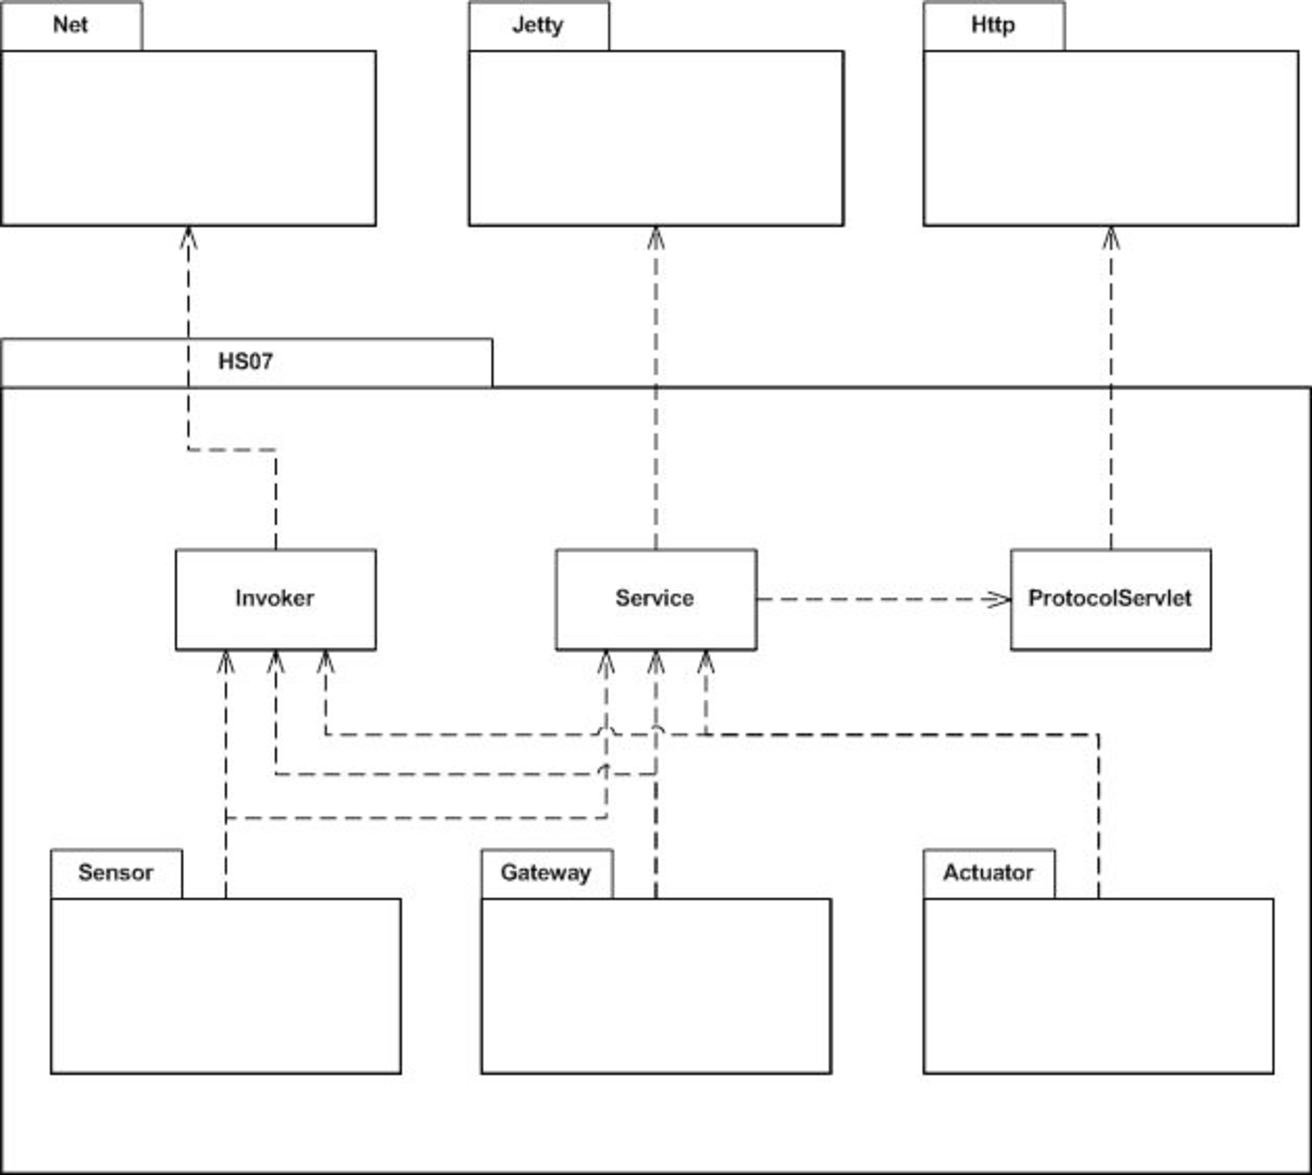
\includegraphics[viewport=0 10 600 550,scale=0.4]{figures/mv.pdf}}
\caption{HS07 Package Diagram}
\label{fig:mv}
\end{figure}

The figure shows the packages of the HS07 system, and how they interact 
with java packages used.

% ---------------------------------------------------------------------
\subsection{Component \& Connector Viewpoint}

The Component \& Connecter view consists of an Active Objects diagram and a
sequence diagram. The Active Objects diagram shows the active objects of 
the HS07 system, and how they interact. 

\begin{figure}[!htb]
\center {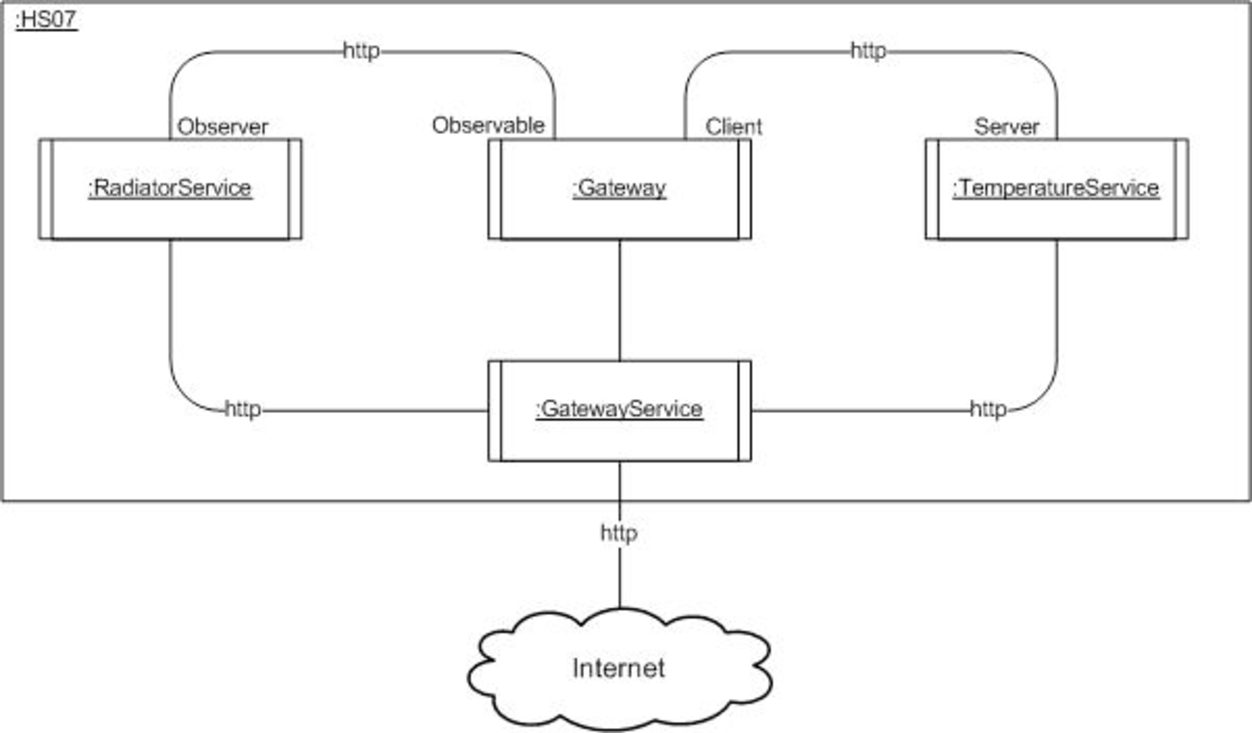
\includegraphics[viewport=0 10 600 420,scale=0.5]{figures/cc_ao.pdf}}
\caption{HS07 Active Objects}
\label{fig:cc_ao}
\end{figure}
The sequence diagram illustrates the timing of the interactions.
\begin{figure}[!htb]
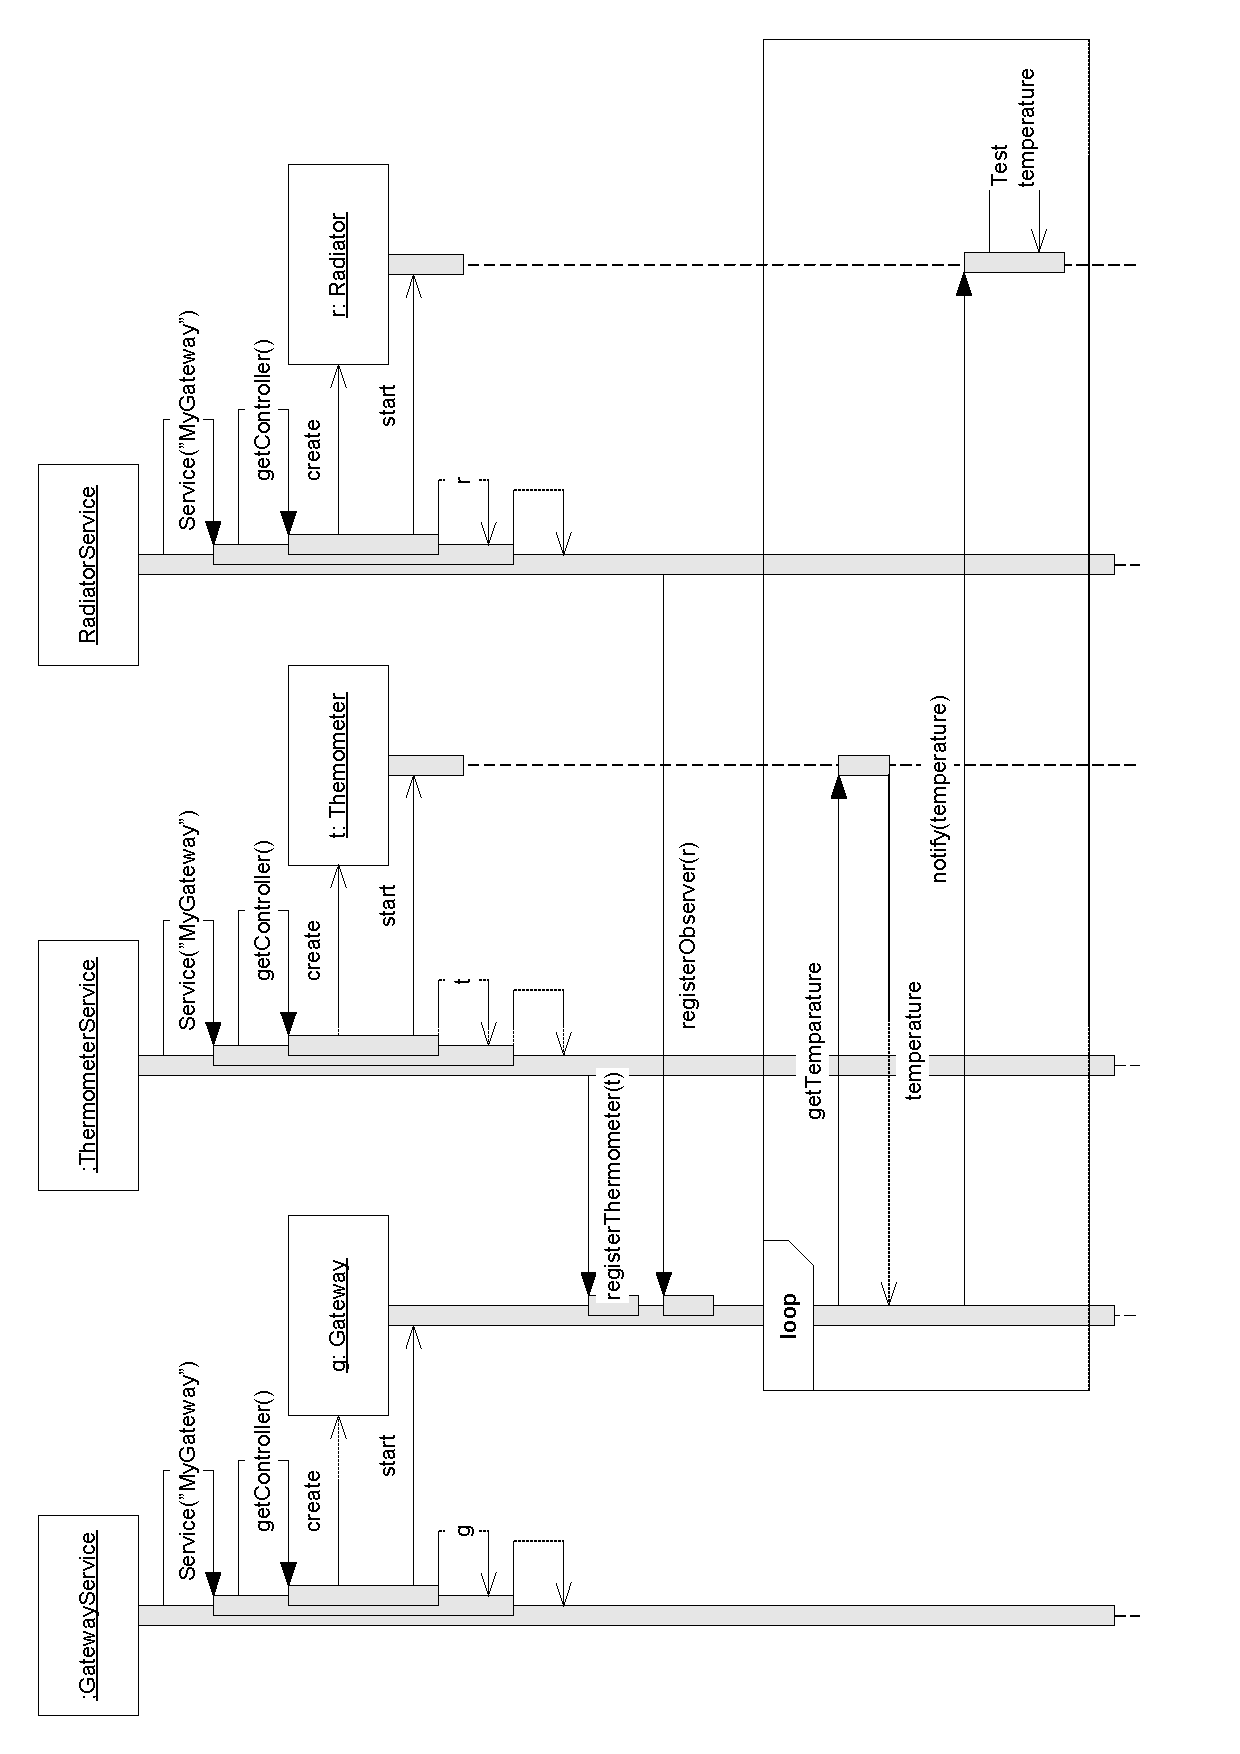
\includegraphics[viewport=0 10 500 650,scale=0.3]{figures/sequence.pdf}
\caption{HS07 Sequence Diagram}
\label{fig:sequence}
\end{figure}


% ---------------------------------------------------------------------
\subsection{Allocation Viewpoint}

The allocation viewpoint illustrates how components are deployed im actaual processes
within the HS07 system.

\begin{figure}[!htb]
\center {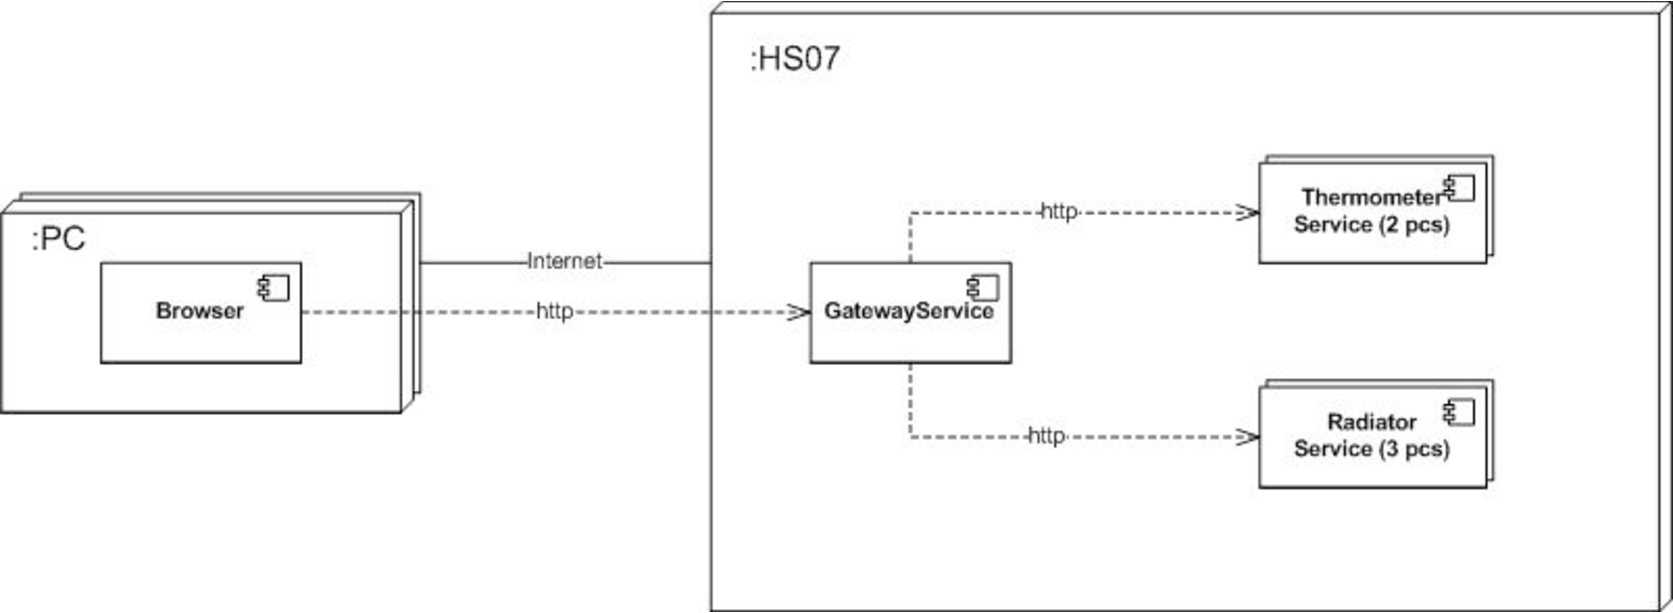
\includegraphics[viewport=0 10 700 350,scale=0.4]{figures/deployment.pdf}}
\caption{HS07 Allocation Diagram}
\label{fig:allocation}
\end{figure}


% =====================================================================
\section{Discussion}
$<<$What are the strengths and limitations of this approach to
architectural description judging from this case?$>>$

$<<$Are there aspects of the software architecture that have not been
properly described?$>>$

$<<$...$>>$

% =====================================================================
\section{...}

% =====================================================================
\bibliography{paper}
\bibliographystyle{apalike}


\end{document}


